\documentclass{standalone}
\usepackage{tikz}

\begin{document}\pagestyle{empty}

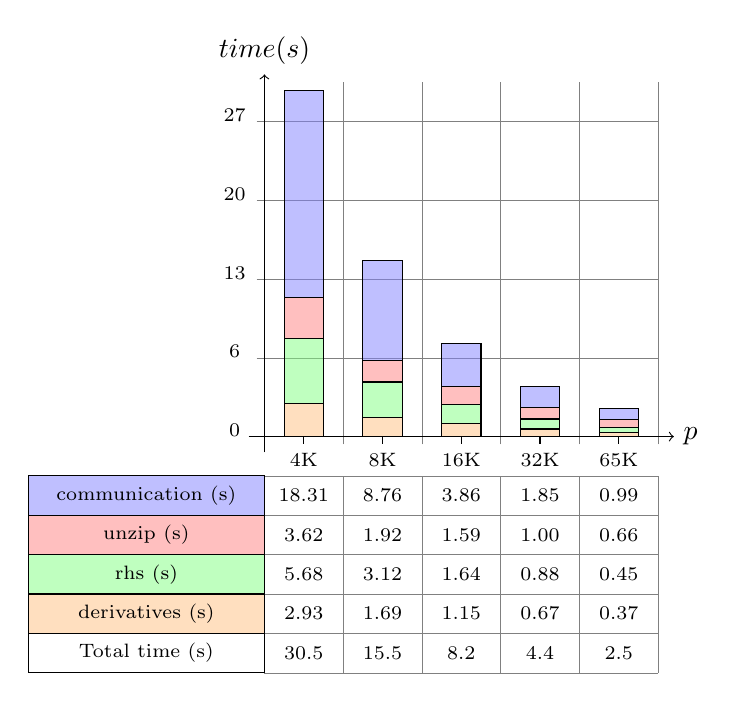
\begin{tikzpicture}

\draw[very thin,color=gray] (-0.1,-0.1) grid (5,4.5);
\draw[->] (-0.2,0) -- (5.2,0) node[right] {$p$};
\draw[->] (0,-0.2) -- (0,4.6) node[above] {$time (s)$};

\foreach \pos/\label in {0.5/4K,1.5/8K,2.5/16K,3.5/32K,4.5/65K}
\draw (\pos,0) -- (\pos,-0.1) (\pos cm,-2.5ex) node [anchor=base,fill=white,inner sep=1pt]  {\scriptsize \label};

\draw[very thin,color=gray, xstep=1, ystep=0.5] (0, -3.0) grid (5,-0.5);
\draw[fill=blue!50, fill opacity=0.5] (-3,-1.0) rectangle +(3,0.5);
\draw (-1.5, -0.75) node {\scriptsize communication (s)};

\draw[fill=red!50, fill opacity=0.5] (-3,-1.5) rectangle +(3,0.5);
\draw (-1.5, -1.25) node {\scriptsize unzip (s)};

\draw[fill=green!50, fill opacity=0.5] (-3,-2.0) rectangle +(3,0.5);
\draw (-1.5, -1.75) node {\scriptsize rhs (s)};

\draw[fill=orange!50, fill opacity=0.5] (-3,-2.5) rectangle +(3,0.5);
\draw (-1.5, -2.25) node {\scriptsize derivatives (s)};

\draw (-3,-3.0) rectangle +(3,0.5);
\draw (-1.5, -2.75) node {\scriptsize Total time (s)};

\draw (-2.5ex, 0 cm) node [anchor=base,fill=white,inner sep=1pt] {\scriptsize 0};

\draw (-2.5ex, 1 cm) node [anchor=base,fill=white,inner sep=1pt] {\scriptsize 6};

\draw (-2.5ex, 2 cm) node [anchor=base,fill=white,inner sep=1pt] {\scriptsize 13};

\draw (-2.5ex, 3 cm) node [anchor=base,fill=white,inner sep=1pt] {\scriptsize 20};

\draw (-2.5ex, 4 cm) node [anchor=base,fill=white,inner sep=1pt] {\scriptsize 27};

\newdimen\mypos
\newdimen\myoff

\foreach \pos/\vala/\valb/\valc/\vald in { 0/18.31/3.62/5.68/2.93, 1/8.76/1.92/3.12/1.69, 2/3.86/1.59/1.64/1.15, 3/1.85/1.00/0.88/0.67, 4/0.99/0.66/0.45/0.37} { 
\mypos=\pos cm
\advance \mypos by 0.5 cm
\draw (\mypos, -0.75 cm) node {\scriptsize \vala};
\draw (\mypos, -1.25 cm) node {\scriptsize \valb};
\draw (\mypos, -1.75 cm) node {\scriptsize \valc};
\draw (\mypos, -2.25 cm) node {\scriptsize \vald};

\myoff=0 cm

\advance \mypos by -0.25 cm
\draw[fill=orange!50, fill opacity=0.5, yscale=0.14408844410678265] (\mypos,\myoff) rectangle +(0.5,\vald);
\advance \myoff by \vald cm
\draw[fill=green!50, fill opacity=0.5, yscale=0.14408844410678265] (\mypos,\myoff) rectangle +(0.5,\valc);
\advance \myoff by \valc cm
\draw[fill=red!50, fill opacity=0.5, yscale=0.14408844410678265] (\mypos,\myoff) rectangle +(0.5,\valb);
\advance \myoff by \valb cm
\draw[fill=blue!50, fill opacity=0.5, yscale=0.14408844410678265] (\mypos,\myoff) rectangle +(0.5,\vala);
\advance \myoff by \vala cm

}

\draw (0.5, -2.75) node {\scriptsize 30.5};
\draw (1.5, -2.75) node {\scriptsize 15.5};
\draw (2.5, -2.75) node {\scriptsize 8.2};
\draw (3.5, -2.75) node {\scriptsize 4.4};
\draw (4.5, -2.75) node {\scriptsize 2.5};
\end{tikzpicture}
\end{document}
